\documentclass[12pt,a4paper]{article}
\usepackage{cmap}
\usepackage{amsmath}
\usepackage[utf8]{inputenc}
\usepackage[T2A]{fontenc}
\usepackage[english, russian]{babel}
\usepackage[left=2cm,right=2cm,top=2cm,bottom=2cm]{geometry}
\usepackage{indentfirst}


%%% Работа с картинками
\usepackage{graphicx}  % Для вставки рисунков
\graphicspath{{Images/}}  % папки с картинками

\usepackage{caption}
\captionsetup{labelsep=period, labelfont=bf}

\def \TITLE {Отчет о выполнении лабораторной работы №0.0.0}
\def \SUBTITLE {Исследование добротности котов.}
\def \AUTHOR {Выполнил студент группы Я00-000\\ Иванов Иван}
\def \DATE {30 августа 2024 г.}

\begin{document}

\begin{titlepage}
	\centering
	\vspace{5cm}
	{\scshape\large Московский физико-технический институт \\
	(НАЦИОНАЛЬНЫЙ ИССЛЕДОВАТЕЛЬСКИЙ УНИВЕРСИТЕТ)}
	
	\vspace{4cm}
	{\LARGE \TITLE}
	
	\vspace{1cm}
	{\Huge\bf \SUBTITLE }
	
	\vspace{1cm}
	\vfill
	
\begin{flushright}
	{\LARGE \AUTHOR}
\end{flushright}
	

	\vfill

	\DATE
\end{titlepage}

\newpage

\section{Аннотация}
	В данной лабораторной работе изучается физиология и поведение котов. В ходе работы студенты знакомятся с основными аспектами жизни котов, такими как питание, уход за шерстью, игры и социализация. Также рассматриваются вопросы здоровья котов, включая профилактику заболеваний и лечение. 

Студенты проводят практические исследования, которые включают наблюдение за поведением котов в различных ситуациях, а также измерение их физических параметров (вес, рост). Они также получают возможность взаимодействовать с котами, чтобы лучше понять их потребности и особенности характера.

В результате выполнения лабораторной работы студенты приобретают знания о том, как правильно ухаживать за котами, как обеспечить им комфортные условия жизни и как предотвратить возможные проблемы со здоровьем.

\section{Теоретические сведения}
\subsection{Физиология котов}
        Пищеварительная система: коты являются хищниками, поэтому их рацион должен содержать достаточное количество белка.
        Дыхательная система: коты дышат через нос и рот, они обладают развитыми легкими и способны адаптироваться к различным условиям окружающей среды.
        Сердечно-сосудистая система: сердце кота бьется с частотой около 100-150 ударов в минуту, что позволяет ему эффективно перекачивать кровь по организму.
        Нервная система: коты обладают сложной нервной системой, которая позволяет им реагировать на различные стимулы и контролировать свои движения.
        
        В рамках классической теории физиологии котов была получена формула \eqref{cat_weight}, определяющая зависимость сытости кота от времени после последнего приёма пищи.
        
\begin{equation}\label{cat_weight}
F = B \cdot e^{At},
\end{equation}
где $F$ -- сытость кота, $B$ -- начальная сытость (калорийность еды), $A = - \frac1\tau$ -- коэффициент падения, $\tau$ -- среднее время между приёмами пищи, $t$ -- время с последнего приёма пищи в часах.
\subsection{Поведение котов}
        Социализация: коты могут быть как социальными, так и независимыми животными, в зависимости от их характера и воспитания.
        Игры: коты любят играть, особенно с игрушками, которые имитируют добычу. Это помогает им поддерживать физическую активность и развивать навыки охоты.
        Уход за шерстью: коты самостоятельно заботятся о своей шерсти, регулярно вылизываясь. Это помогает им сохранять чистоту и поддерживать здоровье кожи.
\subsection{Здоровье котов}
        Профилактика заболеваний: регулярные ветеринарные осмотры, вакцинация и правильное питание помогают предотвратить многие заболевания.
        Лечение: при возникновении болезни необходимо обратиться к ветеринару для получения соответствующего лечения.
        Уход за зубами: коты подвержены заболеваниям полости рта, поэтому важно следить за состоянием их зубов и десен.
\subsection{Уход за котом}
        Питание: коты нуждаются в сбалансированном рационе, который включает в себя мясо, овощи и витамины.
        Гигиена: регулярное мытье и чистка шерсти помогают поддерживать здоровье кожи и шерсти кота.
        Физическая активность: коты нуждаются в достаточной физической активности для поддержания здоровья и хорошего настроения.

Для прогнозирования длины роста шерсти кота можно использовать следующую эмпирическую формулу:

\begin{equation}\label{cat_wool}
L = \arctg\left( Cn^2 + Dn \right),
\end{equation}
где $L$ -- длина шерсти кота, $n$ -- количество месяцев со дня последней стрижки, $C$ и $D$ -- коэффициенты роста шерсти.

\subsection{Добротность кота}
Добротность кота в классической теории физиологии котов может быть по следующей формуле:
\begin{equation}\label{cat_quality}
Q = \frac{\cos^2(\tau)B}{C\ln(20D)}.
\end{equation}

\section{Экспериментальная установка}
Для проведения лабораторной работы необходима экспериментальная установка, включающая в себя следующие компоненты:
\begin{itemize}
    \item Животное: Кот, выбранный для проведения эксперимента. Он должен быть здоровым и активным, без видимых признаков заболеваний или травм.
    \item Пространство для наблюдения: Место, где будет проводиться наблюдение за котом. Это может быть комната или другое помещение, которое должно быть безопасным и удобным для животного.
    \item Игрушки и предметы для взаимодействия: Различные игрушки и предметы, которые могут использоваться для взаимодействия с котом. Это могут быть мячики, мышки, лазерные указки и другие предметы, которые привлекают внимание кота.
    \item Измерительные инструменты: Для измерения физических параметров кота, таких как вес и рост, могут использоваться весы и рулетка.
    \item Записи и заметки: Блокнот или электронное устройство для записи результатов наблюдений и измерений.
    \item Безопасность: Необходимо обеспечить безопасность как для кота, так и для студентов, проводящих эксперимент. Это может включать в себя ограждение опасных предметов, контроль за детьми и другими домашними животными, а также соблюдение правил гигиены и безопасности.
    \item Ветеринарная помощь: В случае необходимости, должна быть доступна ветеринарная помощь для оказания медицинской помощи коту.
    \end{itemize}


\section{Обработка полученных данных}

\subsection{Определение начальной сытости $B$ и среднего времени $\tau$}

По полученным экспериментальным данным построим график на рис. \ref{fig_1} в осях $(t,~ ln(F))$, логарифмируя формулу \eqref{cat_weight} и построим линейную аппроксимацию:
    \begin{equation}
        \ln(F) = \ln(B) + At.
    \end{equation}

\begin{figure}[h!]
    \begin{center}
    		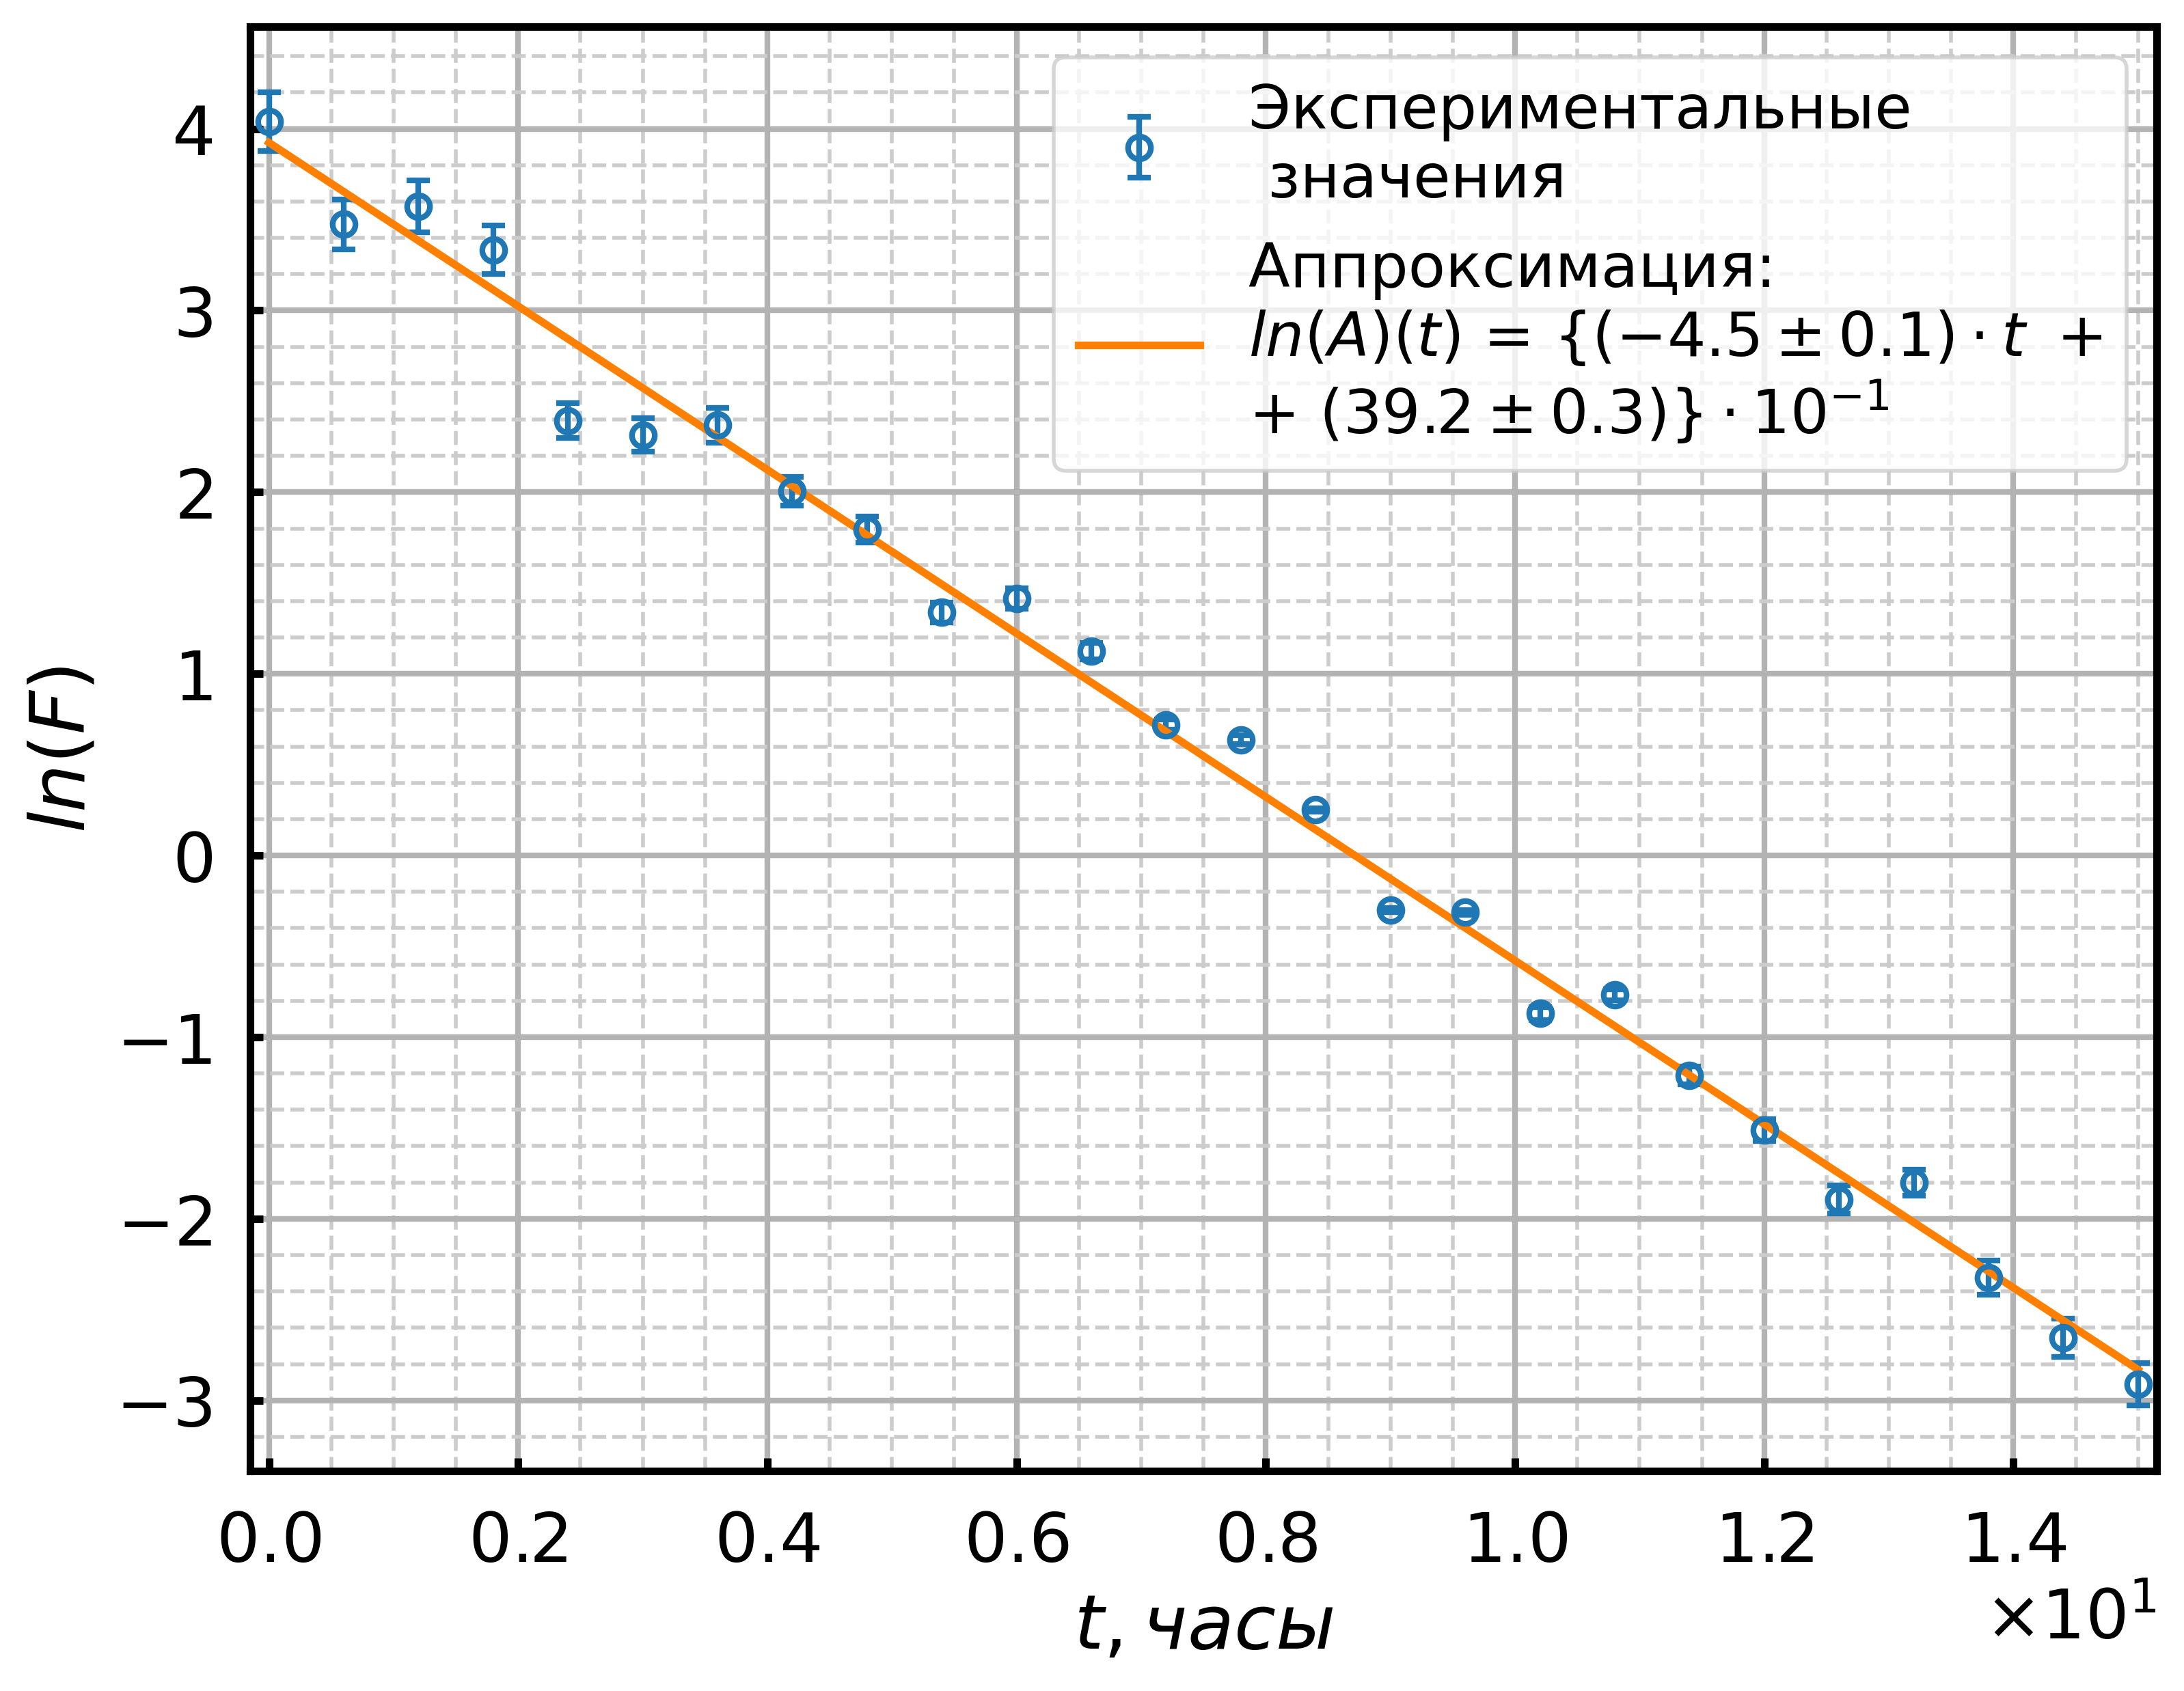
\includegraphics[scale=0.55]{plot_1.png}
    \caption{Зависимость сытости кота от времени в первом эксперименте}\label{fig_1}
    \end{center}
	\end{figure}

Полученные коэффициенты занесём в таблицу:

\begin{table}[h!]
    \centering
    \caption{Коэффициенты $B$ и $\tau$.}\label{table:atau}
	\begin{tabular}{ |c|c|c|}
 \hline
Коэффициент & $B$ & $\tau$ \\
 \hline
 Значение & 50.63 & 2.22 \\ \hline
 Абсолютная погрешность & 0.43 & 0.04 \\ \hline
 Относительная погрешность & 0.01 & 0.02 \\ \hline
	\end{tabular}

\end{table}

\newpage
\subsection{Определение коэффициентов роста шерсти $C$ и $D$}
Преобразуем формулу \eqref{cat_wool}:
\[ \frac{\tg(L)}{n} = Cn + D. \]

Пользуясь этой формулой, построим линейную аппроксимацию графика на рис. \ref{fig_2}, чтобы найти коэффициенты (таблица \ref{table:cd}):

\begin{figure}[h!]
    \begin{center}
    		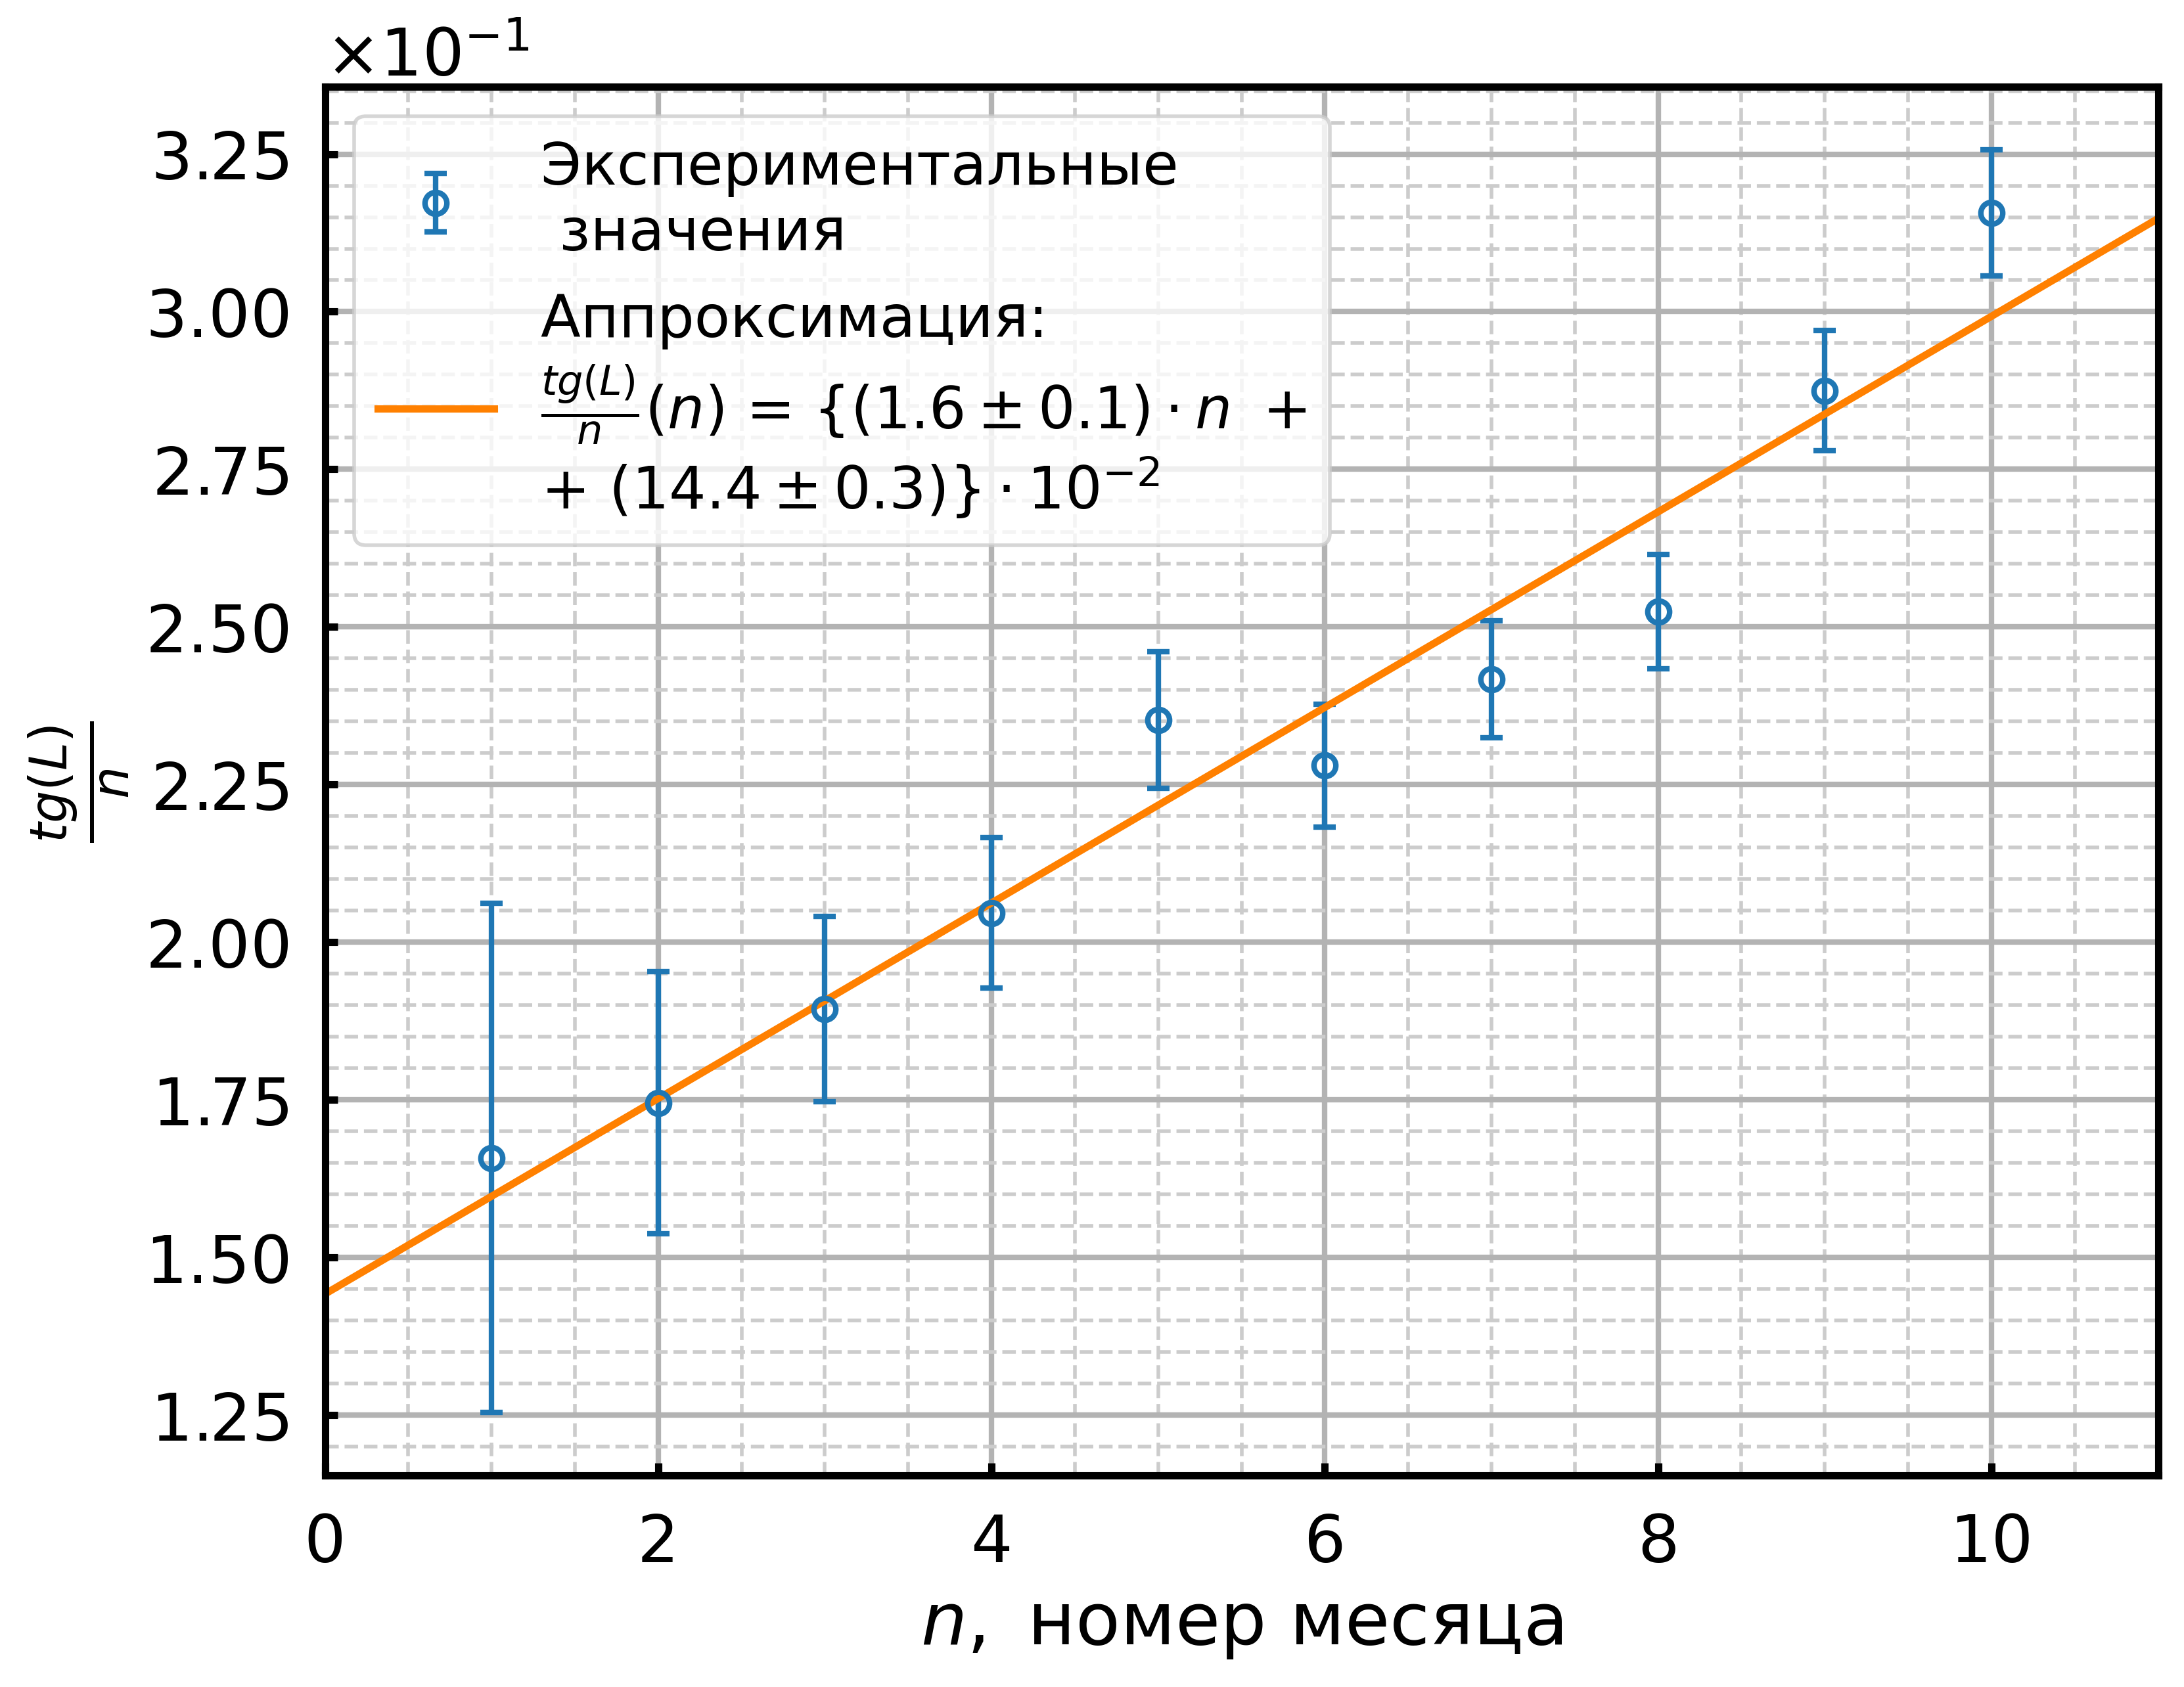
\includegraphics[scale=0.55]{plot_2.png}
    \caption{Зависимость длины шерсти от времени}\label{fig_2}
    \end{center}
\end{figure}

\begin{table}[h!]
    \centering
    \caption{Коэффициенты $C$ и $D$.}\label{table:cd}
	\begin{tabular}{ |c|c|c|}
 \hline
Коэффициент & $C$ & $D$ \\
 \hline
 Значение & 0.0155 & 0.1442 \\ \hline
 Абсолютная погрешность & 0.0011 & 0.0031 \\ \hline
 Относительная погрешность & 0.07 & 0.02 \\ \hline
	\end{tabular}

\end{table}

\subsection{Определение добротности кота}
Пользуясь коэффициентами из таблиц \ref{table:atau} и \ref{table:cd}, а также формулой \eqref{cat_quality}, получим значение добротности рассматриваемого кота:
\[ Q = 1266.1 \pm 88.9 .\]

\section{Выводы.}
\begin{itemize}
    \item Коты обладают высокой добротностью, что проявляется в их способности адаптироваться к различным условиям окружающей среды и сохранять стабильность своего состояния.
    \item Добротность котов связана с их способностью к саморегуляции и адаптации, что позволяет им успешно выживать в различных условиях.
    \item Высокая добротность котов делает их популярными домашними питомцами, поскольку они способны приспосабливаться к различным условиям содержания и образа жизни своих владельцев.
    \item Понимание принципов добротности котов может помочь владельцам создать оптимальные условия для их содержания и ухода, что способствует улучшению качества жизни котов.
    \item Исследование добротности котов является важным шагом в понимании их физиологии и поведения, что может привести к разработке новых методов ухода и лечения этих животных.
\end{itemize}


\end{document}
